\documentclass{beamer}
\usepackage{amsmath}
\usepackage[english]{babel} %set language; note: after changing this, you need to delete all auxiliary files to recompile
\usepackage[utf8]{inputenc} %define file encoding; latin1 is the other often used option
\usepackage{csquotes} % provides context sensitive quotation facilities
\usepackage{graphicx} %allows for inserting figures
\usepackage{booktabs} % for table formatting without vertical lines
\usepackage{textcomp} % allow for example using the Euro sign with \texteuro
\usepackage{stackengine}
\usepackage{wasysym}
\usepackage{tikzsymbols}
\usepackage{textcomp}
% ELIMINAR COMANDOS DE NAVEGACION%%%%%%%%%%%
\setbeamertemplate{navigation symbols}

%% Some commands to make the code easier
\newcommand{\emoticon}[1][]{%
  \node[face,#1] (emoticon) {};
  %% The eyes are fixed.
  \draw[fill=white] (-1ex,0ex) ..controls (-0.5ex,0.2ex)and(0.5ex,0.2ex)..
        (1ex,0.0ex) ..controls ( 1.5ex,1.5ex)and( 0.2ex,1.7ex)..
        (0ex,0.4ex) ..controls (-0.2ex,1.7ex)and(-1.5ex,1.5ex)..
        (-1ex,0ex)--cycle;}
\newcommand{\pupils}{
  %% standard pupils
  \fill[shift={(0.5ex,0.5ex)},rotate=80] 
       (0,0) ellipse (0.3ex and 0.15ex);
  \fill[shift={(-0.5ex,0.5ex)},rotate=100] 
       (0,0) ellipse (0.3ex and 0.15ex);}

\newcommand{\emoticonname}[1]{
  \node[below=1ex of emoticon,font=\footnotesize,
        minimum width=4cm]{#1};}
\usepackage{scalerel}
\usetikzlibrary{positioning}
\usepackage{xcolor,amssymb}
\newcommand\dangersignb[1][2ex]{%
  \scaleto{\stackengine{0.3pt}{\scalebox{1.1}[.9]{%
  \color{red}$\blacktriangle$}}{\tiny\bfseries !}{O}{c}{F}{F}{L}}{#1}%
}
\newcommand\dangersignw[1][2ex]{%
  \scaleto{\stackengine{0.3pt}{\scalebox{1.1}[.9]{%
  \color{red}$\blacktriangle$}}{\color{white}\tiny\bfseries !}{O}{c}{F}{F}{L}}{#1}%
}
\usepackage{fontawesome} % Social Icons
\usepackage{epstopdf} % allow embedding eps-figures
\usepackage{tikz} % allows drawing figures
\usepackage{amsmath,amssymb,amsthm} %advanced math facilities
\usepackage{lmodern} %uses font that support italic and bold at the same time

\usepackage{tikz}
\usepackage{tcolorbox}

\newtcolorbox{boxA}{
    fontupper = \bf,
    boxrule = 1.5pt,
    colframe = black % frame color
}

\usefonttheme[onlymath]{serif} %set math font to serif ones

\definecolor{beamerblue}{rgb}{0.2,0.2,0.7} %define beamerblue color for later use

%%% defines highlight command to set text blue
\newcommand{\highlight}[1]{{\color{blue}{#1}}}


%%%%%%% commands defining backup slides so that frame numbering is correct

\newcommand{\backupbegin}{
   \newcounter{framenumberappendix}
   \setcounter{framenumberappendix}{\value{framenumber}}
}
\newcommand{\backupend}{
   \addtocounter{framenumberappendix}{-\value{framenumber}}
   \addtocounter{framenumber}{\value{framenumberappendix}}
}

%%%% end of defining backup slides

%Specify figure caption, see also http://tex.stackexchange.com/questions/155738/caption-package-not-working-with-beamer
\setbeamertemplate{caption}{\insertcaption} %redefines caption to remove label "Figure".
%\setbeamerfont{caption}{size=\scriptsize,shape=\itshape,series=\bfseries} %sets figure  caption bold and italic and makes it smaller


\usetheme{Boadilla}
\usepackage{hyperref}


% --------------------
% Overall information
% --------------------
\title[Economía I]{Economía I \vspace{4mm}
\\ Magistral 4: La elección del individuo y la curva de demanda individual}
\date{}
\author[Riottini]{Franco Riottini}
\vspace{0.4cm}
\institute[]{Universidad de San Andrés} 


\begin{document}

\begin{frame}
\titlepage
\centering
\includegraphics[scale=0.2]{../Figures/logoUDESA.jpg} 
\end{frame}

\begin{frame}
\frametitle{¡Retomemos!}
\begin{itemize}
  \item Hasta ahora, hemos visto cómo un individuo toma decisiones de consumo
  \item Dada su restricción presupuestaria, elegía la canasta de consumo que se situaba en la curva de indiferencia más lejana
  \item Luego vimos que sucedía cuando cambiaba el nivel de ingreso y cuando se movía en precio de uno de los bienes (efecto ingreso y efecto sustitución) 
  \item Hoy veremos como esto se traslada a una curva de demanda individual.
\end{itemize}
\end{frame}


\begin{frame}
\frametitle{Así finalizamos}
\begin{center}
\begin{figure}[H]
\renewcommand{\figurename}{Figure}
\begin{center}
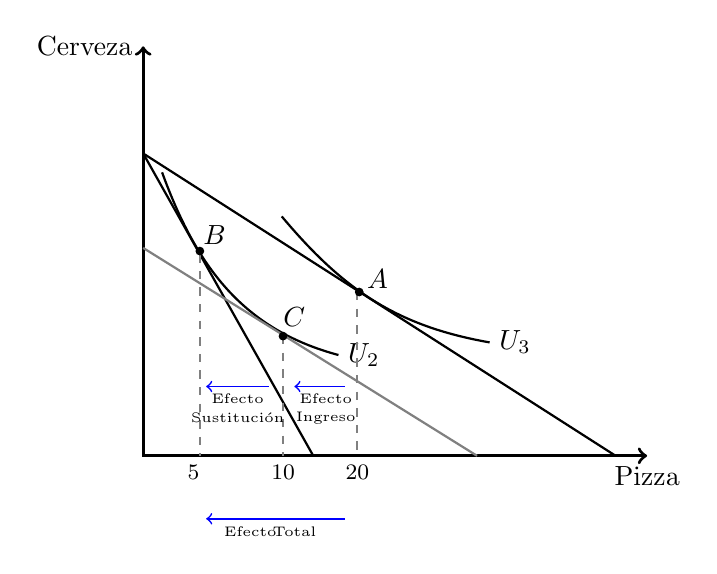
\begin{tikzpicture}[scale=0.8]
\draw[very thick,<->] (0,6.5) node[left]{Cerveza}--(0,0)--(8,0) node[below]{Pizza};
\draw [thick] (2.2,3.8) to [out=310,in=170] (5.5,1.8);
\node [right] at (5.5,1.8) {$U_3$};
\draw [thick] (0.3,4.5) to [out=290,in=165] (3.1,1.6);
\node [right] at (3.1,1.6) {$U_2$};
\node[below] at (3.4,0) {\footnotesize 20};
\node[below] at (2.22,0) {\footnotesize 10};
\node[below] at (0.8,0) {\footnotesize 5};
\draw [thick] (0,4.8) -- (7.5,0);
\draw [thick] (0,4.8) -- (2.7,0);
\draw[thick, dashed,gray](0.9,3.2)--(0.9,0);
\draw[thick, dashed,gray](3.4,2.6)--(3.4,0);
\draw[thick, dashed,gray](2.22,1.9)--(2.22,0);
\draw [thick, gray] (0,3.3) -- (5.3,0);
\draw[semithick, blue, <-] (1,-1)--(3.2,-1);
\node[] at (1.7,-1.2){\tiny Efecto};
\node[] at (2.4,-1.2){\tiny Total};
\draw[semithick, blue, <-] (2.4,1.1)--(3.2,1.1);
\node[] at (2.9,0.9){\tiny Efecto};
\node[] at (2.9,0.6){\tiny Ingreso};
\draw[semithick, blue, <-] (1,1.1)--(2,1.1);
\node[] at (1.5,0.9){\tiny Efecto};
\node[] at (1.5,0.6){\tiny Sustitución};
\node [above] at (2.4,1.9) {$C$};
\draw[fill] (2.22,1.9) circle [radius =0.06];
\node [right] at (0.8,3.5) {$B$};
\draw[fill] (0.9,3.25) circle [radius =0.06];
\node [right] at (3.4,2.8) {$A$};
\draw[fill] (3.43,2.6) circle [radius =0.06];
\end{tikzpicture}
\end{center}
\end{figure}
\end{center}
\end{frame}

\begin{frame}
\frametitle{Cambios en el precio de la pizza}
\begin{itemize}
    \item Si mantenemos constantes el ingreso del individuo y el precio de la cerveza, ¿cómo afectará un cambio en el precio de la pizza a la cantidad de pizza que adquiera el consumidor?
    \begin{itemize}
         \item La canasta de bienes asequible es la que resulta de igualar la pendiente de la curva de indiferencia con la pendiente de la restricción presupuestaria. 
    \end{itemize}
\end{itemize}
\end{frame}

\begin{frame}
\frametitle{Si aumenta el precio de la pizza}
\centering
\includegraphics[scale=0.6]{../Figures/Tema_02.20_rp18.jpg}
\end{frame}

\begin{frame}
\frametitle{El nuevo equilibrio es B}
\centering
\includegraphics[scale=0.6]{../Figures/Tema_02.22_rp20.jpg}
\end{frame}

\begin{frame}
\frametitle{Pensemos un minuto que tenemos aquí...}
\begin{itemize}
    \item Cuando realizamos este ejercicio, estamos obteniendo las cantidades del bien que el individuo está dispuesto a consumir (dado su presupuesto) a cada precio...
    \item Entonces si repetimos el ejercicio varias veces, podríamos ver qué sucede con las cantidades demandadas del consumidor cada vez que el precio aumenta un poquito más.
\end{itemize}
\end{frame}

\begin{frame}
\frametitle{Repitamos el ejercicio de pensar que sucede si cambian los precios... primero el precio es \$50}
\begin{center}
  \begin{minipage}{0.48\textwidth}
      \includegraphics[width=\linewidth]{../Figures/C8.11.png}
  \end{minipage}\hfill
  \begin{minipage}{0.48\textwidth}
      \includegraphics[width=\linewidth]{../Figures/C8.12.png}
  \end{minipage}
\end{center}
\end{frame}

\begin{frame}
\frametitle{Ahora el precio es \$100:}
\begin{center}
  \begin{minipage}{0.48\textwidth}
      \includegraphics[width=\linewidth]{../Figures/C8.13.png}
  \end{minipage}\hfill
  \begin{minipage}{0.48\textwidth}
      \includegraphics[width=\linewidth]{../Figures/C8.14.png}
  \end{minipage}
\end{center}
\end{frame}

\begin{frame}
\frametitle{Y si seguimos aumentando de a \$50...}
\begin{center}
  \begin{minipage}{0.48\textwidth}
      \includegraphics[width=\linewidth]{../Figures/C8.15.png}
  \end{minipage}\hfill
  \begin{minipage}{0.48\textwidth}
      \includegraphics[width=\linewidth]{../Figures/C8.16.png}
  \end{minipage}
\end{center}
\end{frame}

\begin{frame}
\frametitle{Y si seguimos asi...¡¡¡Obtenemos la curva de demanda del estudiante!!!}
\begin{center}
  \begin{minipage}{0.48\textwidth}
      \includegraphics[width=\linewidth]{../Figures/C8.17.png}
  \end{minipage}\hfill
  \begin{minipage}{0.48\textwidth}
      \includegraphics[width=\linewidth]{../Figures/C8.18.png}
  \end{minipage}
\end{center}
\end{frame}

\begin{frame}
\frametitle{¿Cómo pasamos de la curva de demanda individual a la curva de demanda del mercado?}
  \begin{boxA}
    \begin{center}
      \textbf{La demanda individual} es la cantidad de un bien que un individuo está dispuesto a comprar a cada precio.
    \end{center}
  \end{boxA}
\end{frame}

\begin{frame}
\frametitle{Curva de demanda del mercado}
\centering
\includegraphics[scale=0.6]{../Figures/Tema_02.58_demanda.png}
%C10_4.jpg
\end{frame}

\begin{frame}
\frametitle{¿Qué es la demanda?}
\begin{itemize}
    \item La curva de demanda muestra cuál es la disposición máxima a pagar de los consumidores para cada cantidad del bien, o \vspace{2mm}
    \item ... cuál es la cantidad máxima del bien que está dispuesto a consumir el individuo a cada precio.
    \begin{boxA}
      \begin{center}
        ¿Cuales son los factores que afectan a la función de demanda? \\
        Leer capítulo 10 sin falta!
      \end{center}
    \end{boxA}
\end{itemize}
\end{frame}

\begin{frame}
\frametitle{¿Cómo se determina el ingreso?}
\begin{itemize}
    \item Hasta el momento, asumíamos que  conocíamos el ingreso sin preguntarnos como se obtenía. 
    \item Ahora vamos a utilizar las herramientas aprendidas para explicar cómo un individuo determina su ingreso laboral.
    \item A su vez, entender la decisión ocio-trabajo nos será de gran utilidad en la sección de macroeconomía. 
\end{itemize}
\end{frame}


\begin{frame}
\frametitle{Problema consumo - ocio}
\begin{itemize}
    \item Vamos a analizar cómo un individuo decide cuántas horas querrá trabajar por día y, eso definirá su ingreso.
    \item Enfrenta un trade off entre dos bienes: las horas de tiempo libre y el consumo en bienes.
    \item Hay un límite físico: la cantidad de horas por día que puede trabajar o disfrutar.
    \begin{equation}
     24 = H_{Ocio} + H_{Trabajo}.
    \end{equation}
    \item El costo de oportunidad del tiempo libre es el salario. 
    \item El consumo se define por la cantidad de horas de trabajo multiplicado por el salario:
    \begin{equation}
    Consumo = (24-H_{Ocio}) * Salario. 
    \end{equation}
\end{itemize}
\end{frame}


\begin{frame}
\frametitle{Gráficamente..}
\begin{center}
  \includegraphics[scale=0.5]{../Figures/C9.1.png}
\end{center}
\end{frame}

\begin{frame}
\frametitle{La TMT en el modelo ocio - consumo}
  \begin{center}
    \includegraphics[scale=0.45]{../Figures/C9.2.png}
  \end{center}
\end{frame}

\begin{frame}
  \frametitle{La TMS en el modelo ocio - consumo}
  \begin{center}
    \includegraphics[scale=0.5]{../Figures/C9.3.png}
  \end{center}
\end{frame}

\begin{frame}
\frametitle{El equilibrio}
\begin{center}
\includegraphics[scale=0.6]{../Figures/C9.4.png}
\end{center}
\end{frame}


\begin{frame}
\frametitle{¿Por qué G no es un equilibrio?}
\begin{center}
  \includegraphics[scale=0.5]{../Figures/C9.6.png}
\end{center}
\end{frame}

%AGREGAR SLIDES

% SHOCK DE INGRESO EXTRA FIGURA 9.7

% UN AUMENTO EN EL SALARIO FIGURA 9.8

% EL NUEVO EQUILIBRIO FIGURA 9.9 (EFECTO TOTAL)

% EFECTO INGRESO FIGURA 9.10 (PONER EN GRIS LO QUE NO CORRESPONDE AL EFECTO INGRESO)

% EFECTO SUSTITUCION FIGURA 9.11 (PONER EN GRIS LO QUE NO CORRESPONDE AL EFECTO SUSTITUCION)

% LA CURVA DE OFERTA DE TRABAJO DE LARGO PLAZO
% Texto explicando brevemente que refiera a que se observo en el largo plazo



\end{document}